\chapter{Arquitetura de Software}


%Definições - principais (i.e Garlan and Shaw; Krutchen; IEEE)
%Conceitos fundamentais (comuns na literatura)
%Atributos de qualidade
%Decisões arquiteturais
%Papéis
%Visões arquiteturais
%Estilos arquiteturais

%Contexto
O desenvolvimento de um sistema de software não é uma tarefa simples por conta da complexidade envolvida no processo. Além de lidar com a complexidade inerente ao problema a ser resolvido, devemos nos preocupar em como o software resolve esse mesmo problema. Por esse motivo muitos softwares fracassam, seja por custar muito acima do orçamento, estarem imcompletos ou não solucionarem os problemas como deveriam. Assim um software além de resolver o problema, deve resolvê-lo da forma esperada, satisfazendo atributos de qualidade \cite{germoglio2010fundamentos}.

%Contexto
Conforme a complexidade dos softwares aumentam, surgem adversidades. Os problemas de \textit{design} vão além de algorítmos e estruturas de dados, onde a especificação da estrutura geral do sistema surge como um novo obstáculo \cite{garlan1993introduction}. Visando amenizar problemas como esse, a arquitetura de software tem recebido grande atenção  desde a década passada, já que ela tem auxiliado na obtenção de ótimos resultados quanto ao atendimento de atributos de qualidade \cite{fabricio2009instrumentation}. 

Neste capítulo serão apresentados aspectos da arquitetura, relevantes durante a evolução de um sistema de software. Na seção 4.1 são apresentados os principais conceitos sobre arquitetura do ponto de vista da engenharia de software. Já a seção 4.2 expõe elementos da arquitetura do Ruby on Rails, arcabouço utilizado para o desenvolvimento da plataforma Mezuro.

\section{Arquitetura na Engenharia de Software}

%Definição
Desde a primeira referência em um relatório técnico intitulado \textit{Software Engineering Tecnhiques} \cite{buxton1970software}, na década de 1970, diversos autores buscaram definir o termo arquitetura de software de software.
%
Mary Shaw e David Garlan \cite{shaw1996software}, Philippe Kruchten, Grady Booch, Kurt Bittner, e Rich Reitman afirmam que: Arquitetura de Software engloba o conjunto de decisões significativas sobre a organização de um sistema de software incluindo: i) seleção de elementos estruturais e suas interfaces pelos quais um sistema é composto; ii) comportamento como especificado em colaboração entre esses elementos; iii) composição dos elementos estruturais e comportamentais dentro de um subsistema maior; iv) um estilo arquitetural que orienta essa organização. Arquitetura de Software também envolve funcionalidade, usabilidade, flexibilidade, desempenho, reuso, compreensibilidade, restrições econômicas e tecnológicas, vantagens e desvantagens, além de preocupações estéticas.
%Definição da ISO 1471
Com o intuito de estabelecer um padrão sobre o que é e para que serve a arquitetura de software, a ISO 1471 estabelece que Arquitetura de Software é a organização fundamental de um sistema incorporada em seus componentes, seus relacionamentos com o ambiente, e os princípios que conduzem seu design e evolução.
%Elementos básicos
Em suma, há três conceitos citados por todos os autores quando se trata de arquitetura de software \cite{dias2000software}:

\begin{itemize}
\item Elementos estruturais ou de software, também chamados de módulos ou componentes, são as abstrações responsáveis por representar as entidades que implementam funcionalidades especificadas.
\item Interfaces ou relacionamentos, também chamados de conectores, são as abstrações responsáveis por representar as entidades que facilitam a comunicação entre os elementos de software.
\item Organização ou configuração que consiste na forma como os elementos de software e conectores estão organizados.
\end{itemize}

%Atributos de qualidade
Durante a especificação da arquitetura é importante ter a atenção nos relacionamentos entre seus elementos. Essas relações especificam a comunicação, o controle da informação e o comportamento do sistema. Consequentemente, essas relações impactam nos atributos de qualidade, sejam os percebidos pelos usuários, ou apenas pelos desenvolvedores \cite{germoglio2010fundamentos}.
%
Os atributos de qualidade são uma das principais preocupações da arquitetura. Eles representam a maneira que o sistema executará suas funcionalidades e são impostos pelos diversos envolvidos no sistema. Podem ser de três tipos:

\begin{itemize}
\item Atributos de produto ditam como o sistema irá se comportar. Exemplos clássicos são: desempenho, disponibilidade, manutenbilidade, escalabilidade, disponibilidade e portabilidade;
\item Atributos organizacionais são padrões ou regras impostas por organizações envolvidas para satisfazer determinados requisitos. 
\item Atributos externos são leis impostas sobre softwares ou requisitos de interoperabilidade entre sistemas.
\end{itemize}

%TODO: referência

%Decisões Arquiteturais
%TODO: referência
Para satisfazer esses atributos a arquitetura não pode ter suas estruturas definidas aleatoriamente. É necessário que o engenheiro de software opte por alternativas, divida o sistema em elementos e defina seus relacionamentos para alcançar os atributos de qualidade desejados. Esse conjunto de decisões é conhecido por decisões arquiteturais.
%Rastreabilidade
%TODO: referência
Qualquer software possui arquitetura, independente dela ser documentada ou projetada. Entretando, uma arquitetura apenas implementada, ou seja, arquitetura sem projeto, não fornece benefícios ou vantagens que uma arquitetura projetada e bem documentada pode oferecer. Entre os benefícios da documentação da arquitetura estão: i) arquitetura como ferramenta de comunicação entre os participantes do projeto; ii) um método ou modelo para a análise antecipada do sistema a ser desenvolvido; iii) ferramenta de rastreabilidade entre os requisitos e os elementos que compõem o sistema, o que é de grande relevância dada a volatilidade dos requisitos durante o processo de desenvolvimento.
%
Além da participação no desenvolvimento e o estudo da nova arquitetura do Mezuro,
neste trabalho, também colaboraremos com documentação de sua arquitetura, e de modo
que possa ser mantida de acordo com as práticas das comunidades de software livre,
ou seja, também mantida e distruída junto ao código no seu repositório.


%-----------------------parágrafos desconexos---------------------------------------%
% TODO: reescrever por está blabla...
%Por relacionar atributos de qualidade (requisitos não-funcionais) a elementos arquiteturais as decisões auxiliam o rastreameto de requisitos.

%Analisando o ciclo de desenvolvimento de software, é observado que a arquitetura é uma abordagem empregada desde as fases iniciais do processo. Neste instante o nível de abstração da arquitetura é bastante elevado, tendo o objetivo de definir e apresentar a solução computacional que será implementada, auxiliando a tomada de decisões dos stakeholders ou envolvidos no processo de desenvolvimento. Contudo, ao longo do desenvolvimento do software, a arquitetura sofre refinamentos que diminuem o nível de abstração e permitem, por exemplo, a representação dos relacionamentos entre os elementos arquiteturais e os arquivos de código fonte responsáveis por implementá-los \cite{clements2002documenting}.
%---------------------------------------------------------------------------------------%

\section{O arcabouço Ruby on Rails}

O Ruby on Rails é um \textit{arcabouço}, disponível como software livre, criado em 2003 por David Heinemeier Hansson.
%
Sua primeira versão foi lançada em 2004, e desde então seu desenvolvimento e utilização são cada vez maiores.
%
Diversos programadores e empresas em todo mundo utilizam esse o Rails para construirem suas aplicações. Entre as mais conhecidas estão o Twitter (nas primeiras versões), GitHub e Groupon. 
%
O Rails utiliza a linguagem de programação Ruby, criada no Japão em 1995 por Yukihiro "Matz" Matsumoto. A linguagem Ruby é interpretada, multiparadigma, com tipagem dinâmica e gerenciamento de memória automático. O Rails é basicamente uma biblioteca Ruby ou \textit{gem} e é construído utilizando o padrão arquitetural MVC.

Um de seus fundamentos é facilitar o desenvolvimento. O Rails utiliza diversos princípios para orientá-lo do "modo certo" ("Rails way"), possibilitando concentrar esforços no problema do cliente, poupando a equipe do esforço de organizar a estrutura da aplicação a qual é feita pelo arcabouço. Alguns princípios são:

\begin{itemize}

\item \textbf{DRY} - “Don’t Repeat Yourself” - Propõe que um mesmo trecho ou porção de
conhecimento em um código deve possuir representação única no sistema, livre de
redundância e repetições. Quando aplicado, esse princípio possibilita que uma alteração
seja feita em um único local no código, evitando “bad smells” como código duplicado e
facilitando a manutenbilidade do sistema.

\item \textbf{Convenção ao invés de Configuração} (Convention over configuration)- Considerado um paradigma de design que visa diminuir o número de decisões que os desenvolvedores precisam tomar, ganhando simplicidade, sem perder simplicidade.

\item \textbf{REST} - É um estilo arquitetural para aplicações web. O termo REST é um acrônimo para \textbf{RE}presentaional \textbf{S}tate \textbf{T}ransfer. Propõe princípios (não exclusivos ao REST) que definem como Web Standards como HTTP e URIs devem ser usados. Os princípios são:

  \begin{itemize}

  \item Todos os recursos devem ter um identificador. Um conceito comum para identificador na web é a URI;

  \item Utilize links (hipermídia) para referenciar recursos;

  \item Utilize os métodos padrão - São eles GET, POST, PUT, DELETE. Os métodos GET e PUT e DELETE são idempotentes, ou seja, há garantia de que podemos enviar a requisição novamente. Quando emitimos um GET, por exemplo, e não recebermos resposta, não saberemos se a requisição foi perdida ou a resposta que se perdeu. Mas nesse caso podemos simplesmente enviar a solicitação novamente;

  \item Múltipla representação de recursos - diversos formatos dos recursos para diferentes necessidades, como formatos XML, HTML. Isso faz com que seus recursos sejam consumidos não apenas pelo seu aplicativo, mas também por qualquer navegador web;

  \item Comunicação sem estado - Um servidor não deveria guardar o estado da comunicação de qualquer um dos clientes que se comunique com ele além de uma única requisição. A razão para isso é escalabilidade - o número de clientes que podem interagir com o servidor seria consideravelmente impactado se fosse preciso manter o estado do cliente;

  \end{itemize}
\end{itemize}

%TODO: não tem nenhuma referência para nada o que você falou até aqui...
% Não foi você que inventou isso tudo, tem que dar o crédito a quem definiu ;)

%---------------------------------------------------------------------------------------%

\subsection{Evolução do Ruby on Rails}
\label{sec:rails}

O arcabouço Rails, desde seu lançamento, sofre frequentes alterações, e com isso novas versões são lançadas constantemente, conforme apresentado na Tabela~\ref{tab:rails_versions}. Muitos desenvolvedores enxergam essas constantes mudanças como um ponto negativo, ao passo que há incompatibilidade de algumas "gems" de uma versão para outra. Por outro lado, outros aprovam essa característica pois a cada atualização há melhora no produto, com adição de novos recursos, além de ser um incentivo para a implementação de testes, já que eles auxiliam a manter a integridade da aplicação a cada atualização.

\begin{table}[H]
\begin{center}
    \begin{tabular}{ | l | l |}
    \hline
    Versão & Data \\ \hline
    1.0 & 13/12/2005 \\ \hline
    1.2 & 19/01/2007 \\ \hline
    2.0 & 7/12/2007 \\ \hline
    2.1 & 01/06/2008 \\ \hline
    2.2 & 21/11/2008 \\ \hline
    2.3 & 16/03/2009 \\ \hline
    3.0 & 29/08/2010 \\ \hline
    3.1 & 31/08/2011 \\ \hline
    3.2 & 20/01/2012 \\ \hline
    4.0 & 25/06/2013 \\ \hline
    \end{tabular}
    \caption{Versões do Rails}
    \label{tab:rails_versions}
\end{center}
\end{table}

Entre os novos recursos oferecidos pela versão 4 do Rails, que é a versão usada no novo Mezuro, estão:

\begin{itemize}

	\item Páginas mais rápidas através da utilização de Turbolinks. Ao invés de deixar o navegador recompilar o JavaScript e CSS entre cada mudança de página, a instância da página atual é mantida, substituindo apenas o conteúdo e o título.

	\item Suporte para a expiração de cache baseado em chave, que automatiza a invalidação do cache e deixa mais fácil a implementação de estruturas de cache sofisticadas.

	\item Streaming de vídeo ao vivo em conexões persistentes.

	\item Melhorias no ActiveRecord para aprimorar a consistência do escopo e da estrutura das queries.

	\item Padrões de segurança locked-down.

	\item Threads seguras por padrão e a eliminação da necessidade de configurar servidores com thread.

\end{itemize}

%TODO: também se referencia ou coloca-se uma nota de rodapé de onde o leitor pode ver isso e conhecer mais a tecnologia.

%---------------------------------------------------------------------------------------%

\subsection{Padrao Arquitetural MVC}

O padrão MVC começou como um arcabouço desenvolvido por Trygve Reenskaug para a plataforma SmallTalk, no final dos anos 70. Desde então, ele exerce grande influência sobre diversos arcabouços que promovem interação com usuário, como é o caso do Ruby on Rails.
%
O MVC visa separar a representação da informação da interação com o usuário. Para atingir esse objetivo são utilizados três ``papéis'', conforme apresentado do na Figura~\ref{fig:mvc}:
%
(i) O modelo (\textit{model}) que representa informações do domínio, como dados
da aplicação, regras de negócio, lógica e funções;
%
A visão (\textit{view}) que são saídas de representação dos dados do modelo ao
usuário. Um exemplo comum de visão é uma pagína HTML contendo dados presentes
no modelo.
%
O útimo papel, o controlador (\textit{controller}) é responsável por receber
requisições da visão, manipula-las, utilizando dados do modelo, e atualizar a
visão para satisfazer as requisições do usuário.

\graphicspath{{figuras/}}
\begin{figure}[H]
\centering
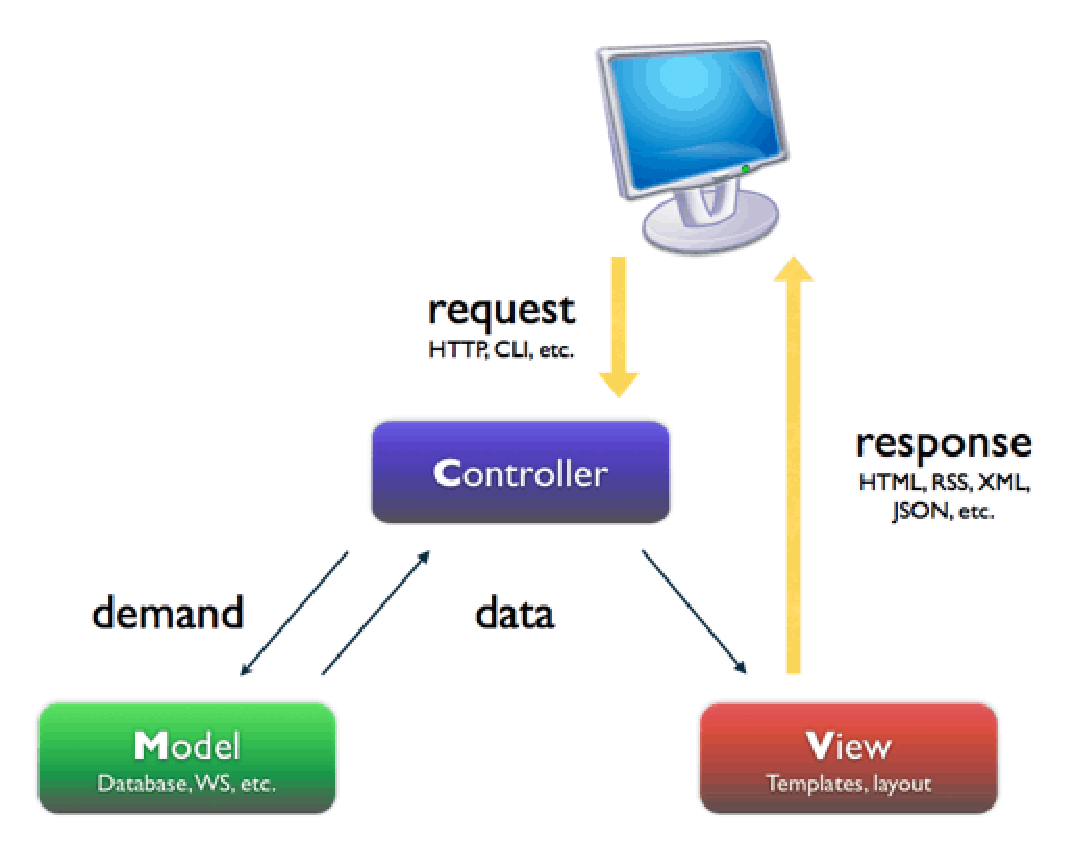
\includegraphics[width=0.5\textwidth]{mvc}
\caption{Representação do padrão MVC}
\label{fig:mvc}
\end{figure}

O exempo abaixo ilustra um cenário de execução de uma funcionalidade com o padrão MVC.

\begin{mdframed}[frametitle={Exemplo},roundcorner=5pt]
Um usuário navega em um site de vendas de veículos. Ao pressionar o botão para visualizar determinado veículo, o navegador carrega a página de detalhes e a devolve ao usuário. Esse processo começa quando na VIEW o usuário pressiona o botão de visualização. A URL gerada é processada por um método da CONTROLLER de veículos. Esse método solicita ao MODEL o veículo correspondente a URL, então a VIEW é renderizada com os dados do veículo correspondente, obtidos pela CONTROLLER.
\end{mdframed}

%TODO: tudo sem referência até aqui...

%---------------------------------------------------------------------------------------%

\subsection{Arquiterura do Rails}

Entre os elementos da arquitetura de software, há elementos estáticos e dinâmicos. Elementos estáticos definem as partes de um sistema e sua organização. Entre elementos estáticos estão: i) elementos de software; ii) elementos de dados; iii) elementos de hardware. 
%
As características do Rails estão distribuídas entre elementos, conforme ilustrado na Figura~\ref{fig:rails-architecture}.
%
Os relacionamentos entre os elementos também estão inclusos, e também compõem o aspecto estático da arquitetura do sistema \cite{germoglio2010fundamentos}.
%
Já os elementos dinâmicos definem o comportamento do sistema e representa o sistema em execução. Nele estão incluídos processos, protocolos, módulos e classes que realizam comportamento.

\graphicspath{{figuras/}}
\begin{figure}[H]
\centering
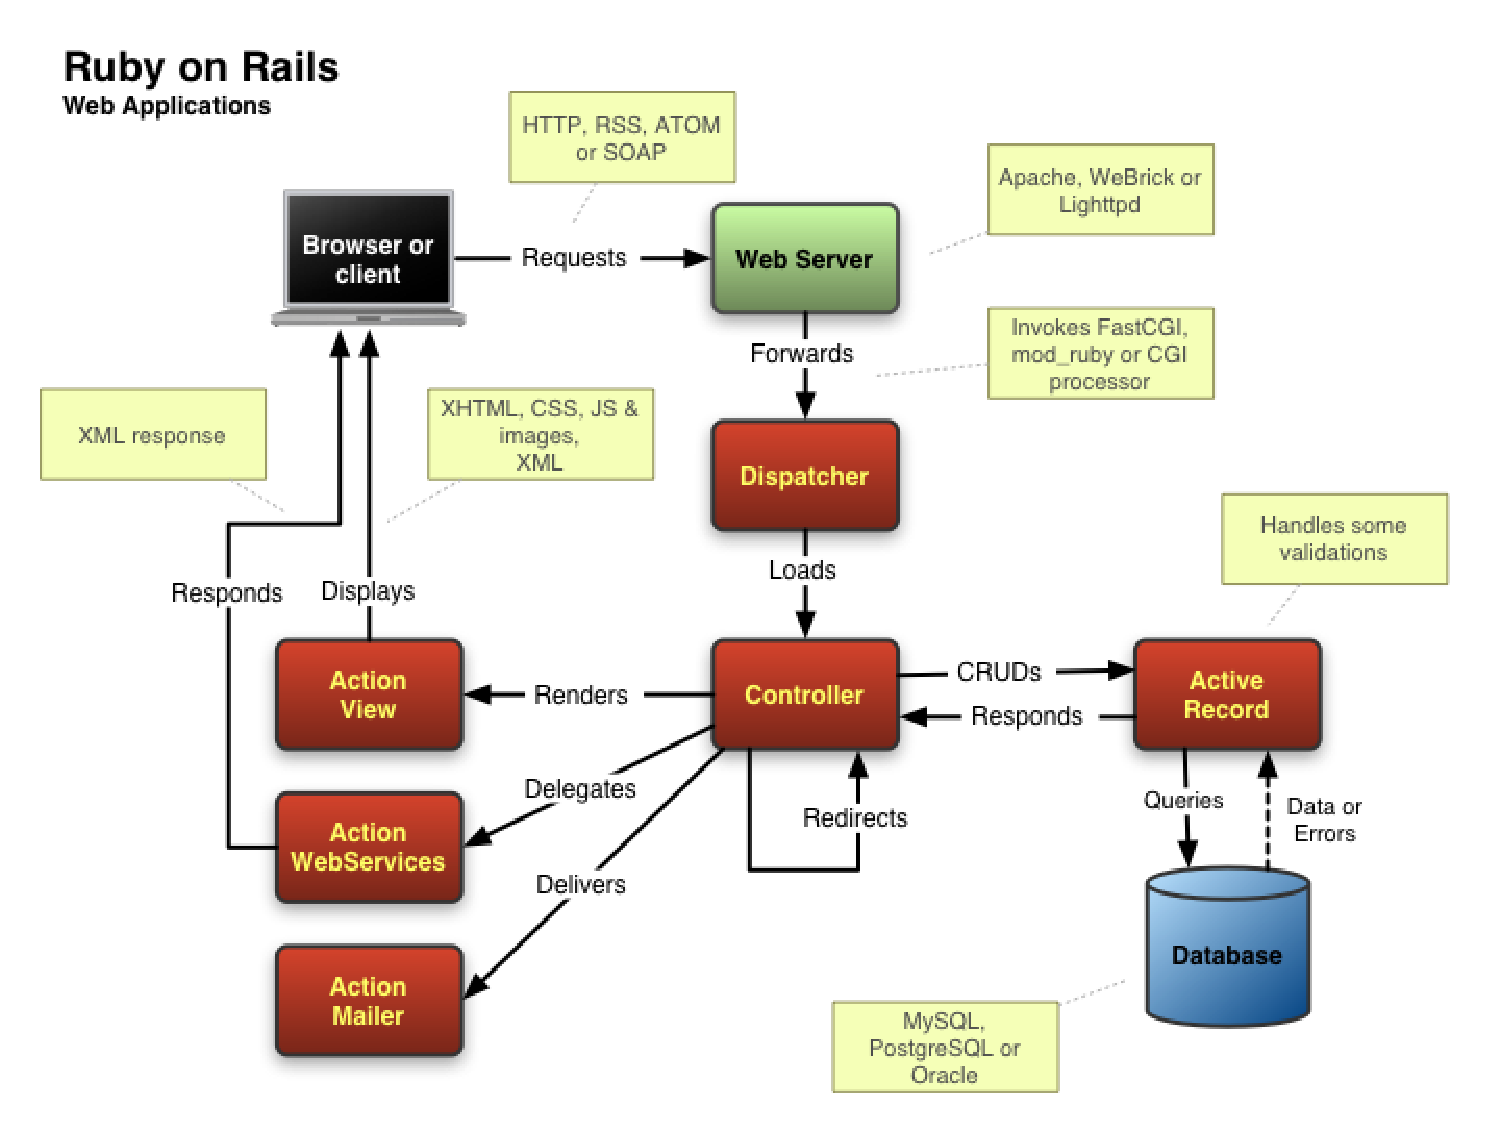
\includegraphics[width=0.7\textwidth]{rails-overview}
\caption{Interação entre os componentes do Rails. Extraído  de \cite{mejia2011rails}}
\label{fig:rails-architecture}
\end{figure}


\begin{description}

\item [Action Mailer] fornece a capacidade de criação de serviços de e-mail. Podendo enviar e-
mails baseados em templates adaptáveis ou receber e processar um e-mail;

\item [Action Pack]

 \begin{description}

	 \item [Action Controller] é o componente que gerencia os controllers em uma aplicação
	Rails. Ele processa as requisições que chegam de uma aplicação Rails, recebe seus
	parâmetros e os envia para as ações pretendidas; 

	 \item [Action View] gerencia as views da aplicação. Isto é, as saídas HTML e XML por
	padrão. Gerencia a renderização de templates aninhados ou parciais , e inclui suporte
	embutido para AJAX;

 \end{description}

\item [Active Record] é abase dos \textit{models}. Ele fornece a independência de banco de dados e CRUD básico. Ele é utilizado para criar a representação, em orientação a objetos, dos
dados presentes no banco de dados;

\item [Active Resource] gerencia conexões entre objetos de negócio e serviços web RESTful.
Ele mapeia recursos baseados em web para objetos locais com lógica CRUD;

\item [Active Support] uma coleção de classes de utilidade e extenções da biblioteca padrão do
Ruby que são utilizadas pelo Rails, tanto em seu núcleo quanto para suas aplicações;

\item [Railties] é o núcleo do código Rails e é ele quem constrói novas aplicações Rails e junta os diversos componentes;

\end{description}


%TODO: concluir algo
